\chapter[Resultados]{Resultados}
\label{sec:resultados}
Neste capítulo, estão descritos os resultados que foram obtidos até o momento de publicação deste trabalho. O capítulo está dividido em apenas uma seção, onde é relatado os resultados que foram alcançados ao final das iterações e o produto final que e o \textit{dashboard}.

\section{Resultados Obtidos}
\label{resultados_obtidos}

Após feito o levantamento bibliográfico começou-se a primeira \textit{sprint} do desenvolvimento da solução, que consistia em implementar a funcionalidades: cadastrar um gestor (sendo que este tivesse como realizar um \textit{login} na aplicação) e cadastrar projetos. Com a implementação feita, realizava-se um teste de usabilidade com um grupo de pessoas. Esse grupo de pessoas consistia em quatro alunos de Engenharia de Software da Universidade de Brasília, sendo dois alunos no último semestre do curso, 1 aluno no quinto período e outro do sétimo período. O teste de usabilidade consistia em uma lista de sete atividades que deveriam ser executadas pelo examinado. Nesse primeiro teste foram pedidos que os examinados realizassem atividades mais simples para se contextualizar com o software e com a finalidade do software. Através do gráfico da Figura \ref{img:grafico_iteracao1}, fica possível perceber que os entrevistados tiveram problema para realizar a ativdade 5. Maiores detalhes quanto ao tempo de cada entrevistado se encontram na Tabela \ref{tabela_iteracao1}.

\graphicspath{{figuras/}}
\begin{figure}[!h]
\centering
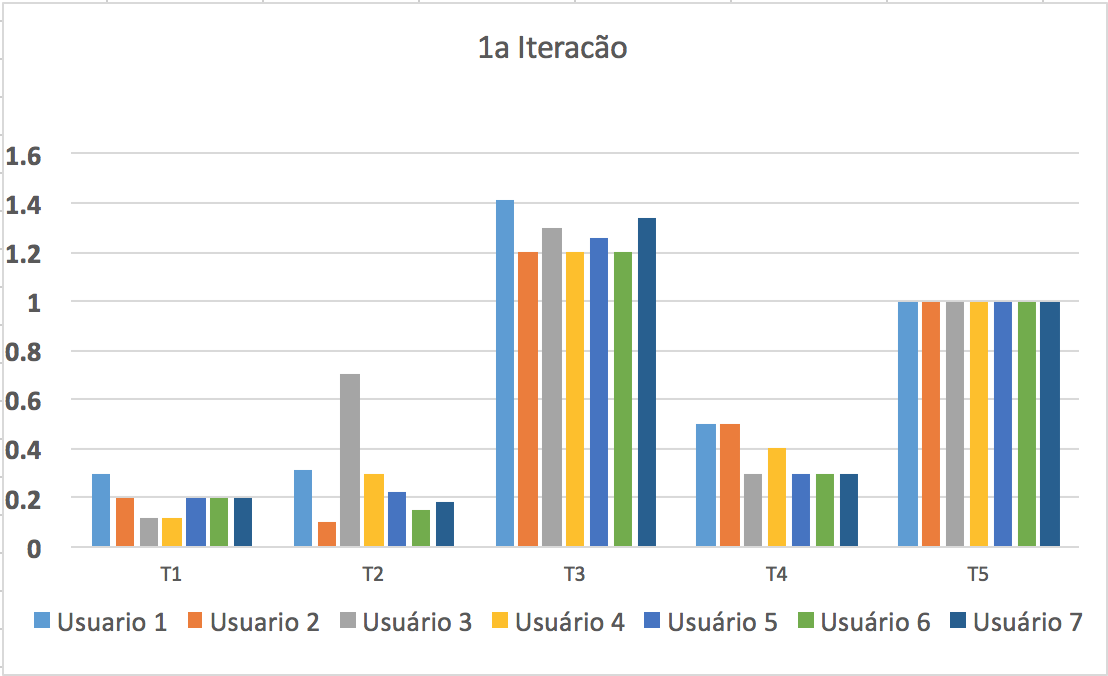
\includegraphics[scale=0.75]{iteracao1_grafico}
\caption{Gráfico Comparativo das Atividades Realizadas na Iteração 1}
\label{img:grafico_iteracao1}
\end{figure}

\begin{table}[h!]
\centering
\caption{Tempo de Execução de Cada Atividade em Segundos 1a Iteração}
\label{tabela_iteracao1}
\begin{tabular}{|llllll|}
\hline
\multicolumn{6}{|c|}{\cellcolor[HTML]{C0C0C0}\textbf{1a Iteracão}}                     \\ \hline
                   & \textbf{T1} & \textbf{T2} & \textbf{T3} & \textbf{T4} & \textbf{T5} \\ \hline
\textbf{Usuário 1} & 0.3         & 0.31        & 1.41        & 0.5         & 1           \\ \hline
\textbf{Usuário 2} & 0.2         & 0.1         & 1.2         & 0.5         & 1           \\ \hline
\textbf{Usuário 3} & 0.12        & 0.7         & 1.3         & 0.3         & 1           \\ \hline
\textbf{Usuário 4} & 0.12        & 0.3         & 1.2         & 0.4         & 1           \\ \hline
\textbf{Usuário 5} & 0.2         & 0.22        & 1.26        & 0.3         & 1           \\ \hline
\textbf{Usuário 6} & 0.2         & 0.15        & 1.2         & 0.3         & 1           \\ \hline
\textbf{Usuário 7} & 0.2         & 0.18        & 1.34        & 0.3         & 1           \\ \hline
\end{tabular}
\end{table}


Após as atividades propostas pelo entrevistador, perguntava-se aos entrevistados quanto à experiencia que eles haviam tido ao utilizar o software. Um dos pontos ressaltados pelos entrevistados foi quanto ao uso de não haver uma descrição quanto a funcionalidade de voltar ao menu utilizando o canto esquerdo superior da tela como pode ser observado na Figura \ref{img:alteracao_menu}. 

\graphicspath{{figuras/}}
\begin{figure}[h!]
\centering
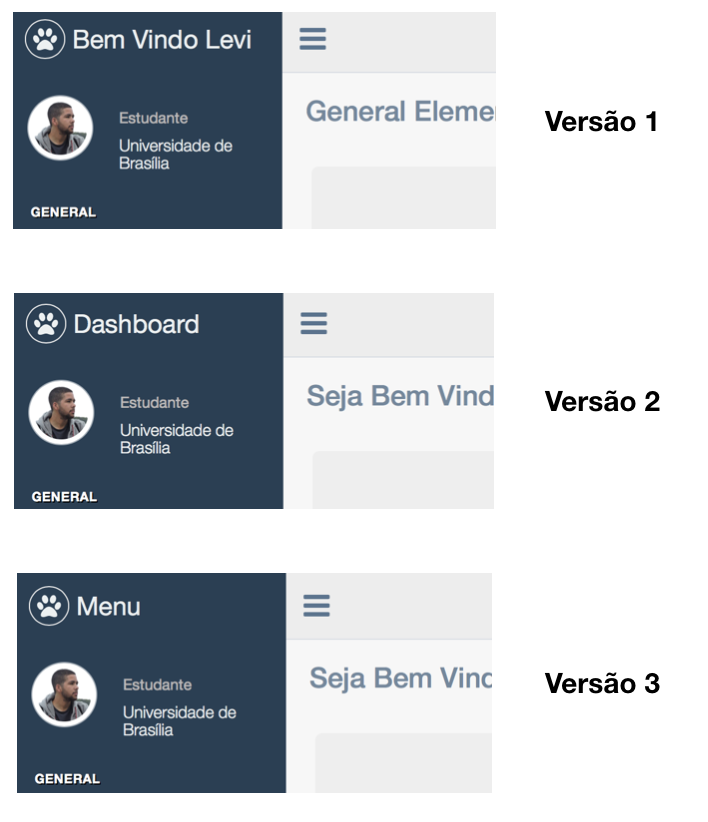
\includegraphics[scale=0.80]{comparacao_versoes_menu}
\caption{Alterações feitas no \textit{link} de menu}
\label{img:alteracao_menu}
\end{figure}

Para a segunda \textit{sprint} decidiu-se elaborar as funcionalidades de acompanhar projeto e exibir métricas. Foram entrevistadas as mesmas pessoas da primeira Iteração e seguiu-se as mesmas atividades da Iteração anterior. Os resultados obtidos estão na Tabela \ref{tabela_iteracao2}. A partir do gráfico presente na Figura \ref{img:grafico_iteracao2} percebe-se que o Usuário 1 apresentou um comportamento fora do esperado, isso se deve ao fato de que o examinado havia se confundido quanto ao enunciado da Tarefa 5.


\begin{table}[h!]
\centering
\caption{Tempo de Execução de Cada Atividade em Segundos 2a Iteração}
\label{tabela_iteracao2}
\begin{tabular}{|llllllll|}
\hline
\multicolumn{8}{|c|}{\cellcolor[HTML]{C0C0C0}\textbf{2a Iteração}}                                                   \\ \hline
                   & \textbf{T1} & \textbf{T2} & \textbf{T3} & \textbf{T4} & \textbf{T5} & \textbf{T6} & \textbf{T7} \\ \hline
\textbf{Usuário 1} & 0.04        & 0.32        & 0.11        & 0.19        & 0.37        & 0.07        & 0.07        \\ \hline
\textbf{Usuário 2} & 0.05        & 0.2         & 0.07        & 0.16        & 0.07        & 0.32        & 0.05        \\ \hline
\textbf{Usuário 3} & 0.05        & 0.17        & 0.05        & 0.14        & 0.08        & 0.27        & 0.02        \\ \hline
\textbf{Usuário 4} & 0.04        & 0.2         & 0.02        & 0.13        & 0.08        & 0.3         & 0.04        \\ \hline
\textbf{Usuário 5} & 0.05        & 0.22        & 0.12        & 0.15        & 0.07        & 0.35        & 0.05        \\ \hline
\textbf{Usuário 6} & 0.05        & 0.24        & 0.16        & 0.16        & 0.07        & 0.26        & 0.05        \\ \hline
\textbf{Usuário 7} & 0.06        & 0.2         & 0.16        & 0.18        & 0.07        & 0.05        & 0.06        \\ \hline
\end{tabular}
\end{table}

\graphicspath{{figuras/}}
\begin{figure}[h!]
\centering
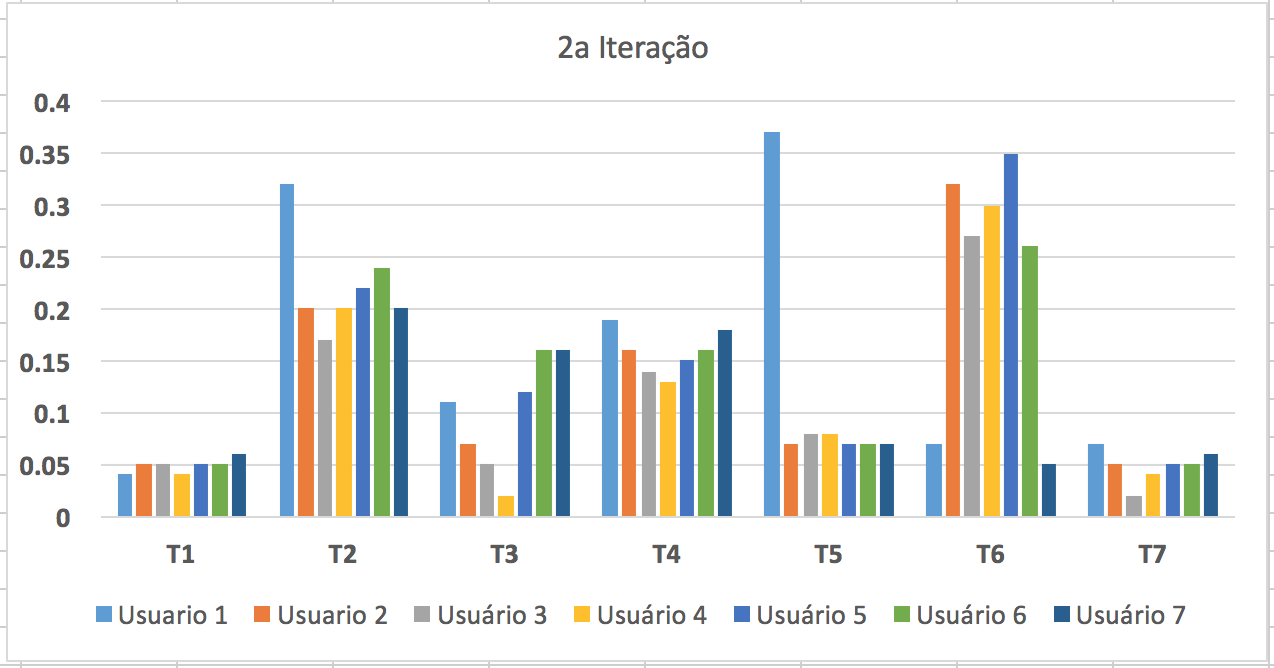
\includegraphics[scale=0.75]{grafico_2a_iteracao}
\caption{Gráfico Comparativo das Atividades Realizadas na Iteração 2}
\label{img:grafico_iteracao2}
\end{figure}

 Uma das mudanças implementadas nessa segunda iteração se deve ao acréscimo de um botão para adicionar projeto na própria pagina inicial da aplicação. Este pedido havia sido feito na 1a Iteração por um dos entrevistados. Está alteração pode ser vista na Figura \ref{img:compara_botao}.
 
 
 \graphicspath{{figuras/}}
 \begin{figure}[h!]
 \centering
 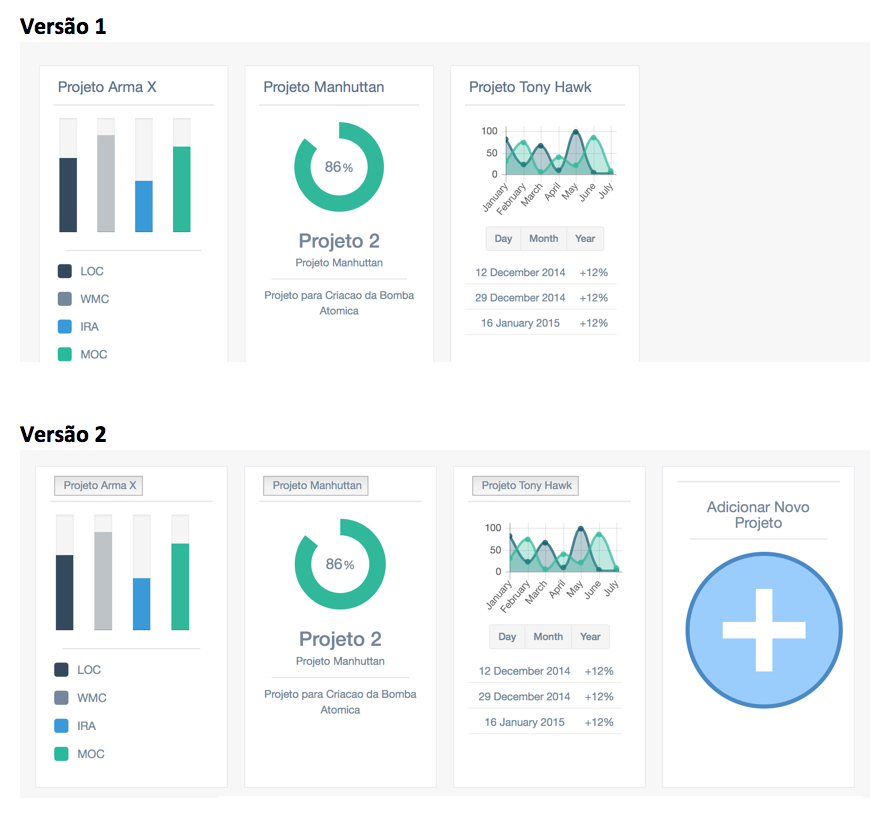
\includegraphics[scale=0.60]{compara_adicao_botao}
 \caption{Acréscimo do Botão de Adicionar Projeto na Página Inicial}
 \label{img:compara_botao}
 \end{figure}
 
Ainda na \textit{sprint} 2, destaca-se o botão para acesso rápido ao cadastro de um novo projeto, que foi um dos pontos levantados pelos entrevistados, presente na Figura \ref{img:pag_inicial}. Outro destaque desta figura está nos \textit{widgets} personalizáveis que apresentam uma visão resumida do estado atual do projeto.

\graphicspath{{figuras/}}
\begin{figure}[h!]
\centering
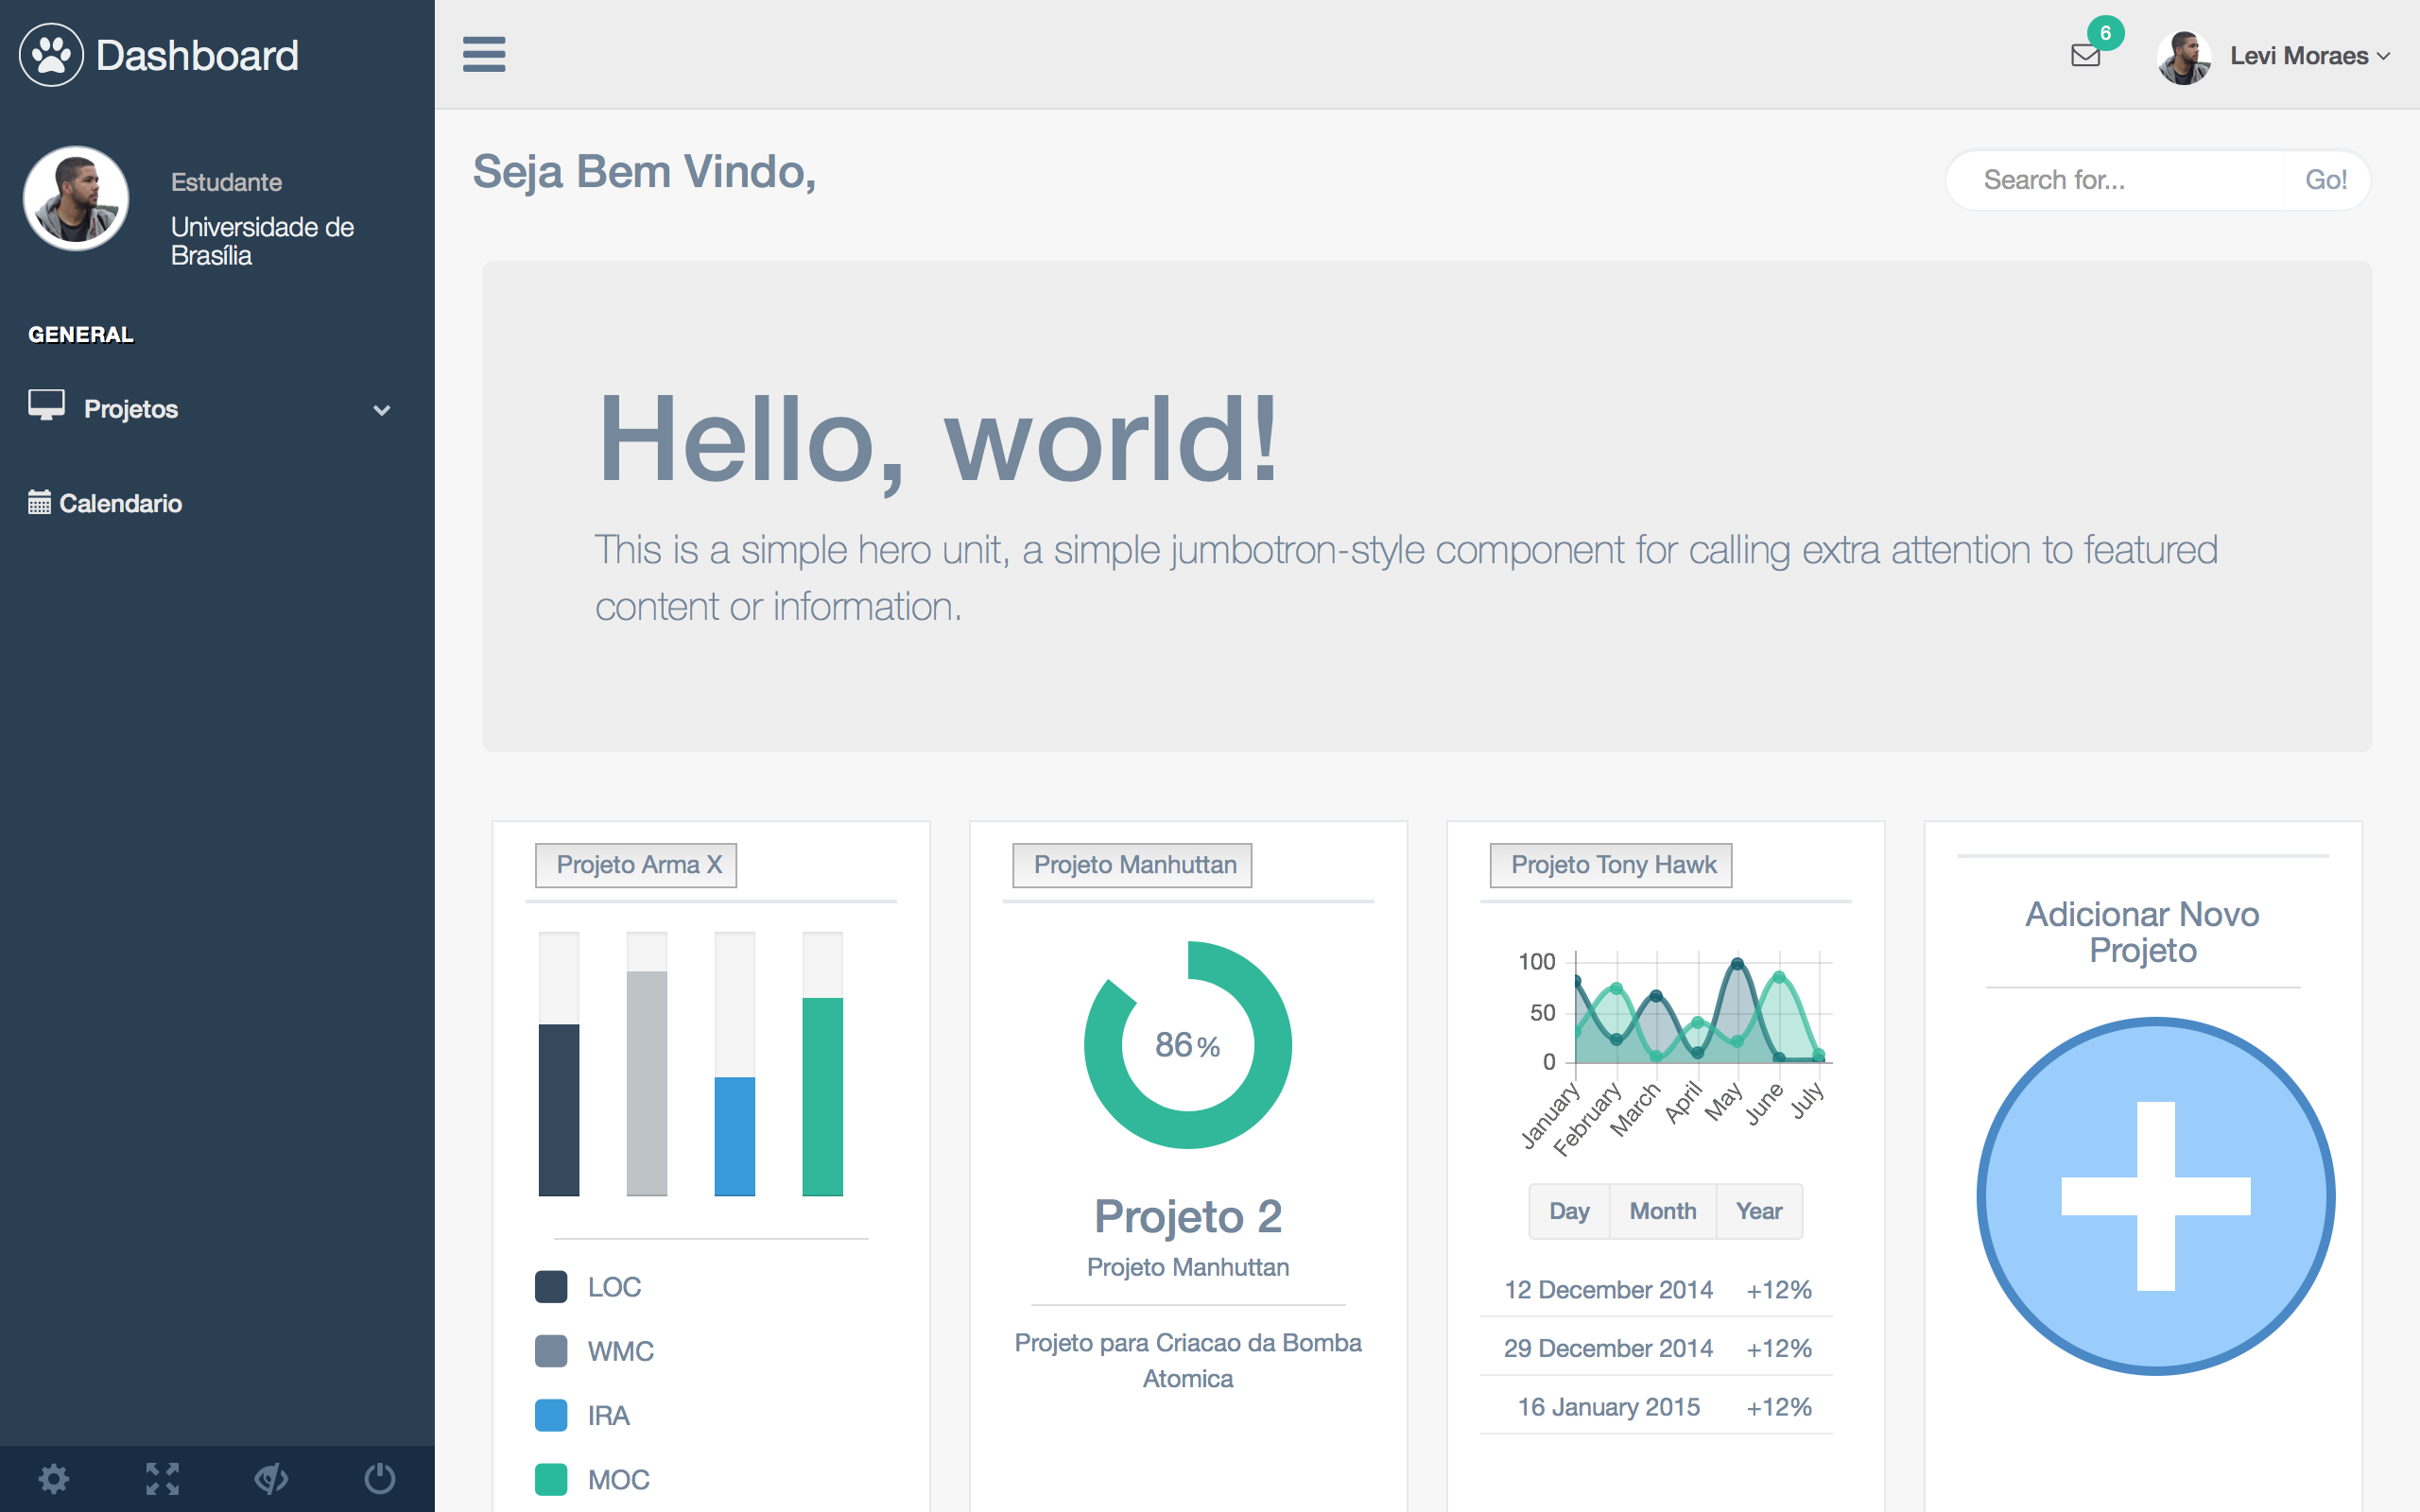
\includegraphics[scale=0.35]{pagina_inicial}
\caption{Página Inicial da Aplicação}
\label{img:pag_inicial}
\end{figure}

A Figura \ref{img:pag_visual} apresenta todos os projetos do gestor, indicando o status de completude do projeto em relação à data de entrega. Percebe-se também a utilização de ícones para representar ações comuns e conhecidas do usuário, como o símbolo do lápis indicando um botão com a funcionalidade de alterar e uma lixeira indicando a ação de exclusão. Ressalta-se também o uso das cores nos botões, em que ações destrutivas (como a exclusão de um projeto), apresenta uma cor de destaque em relação as demais.


\graphicspath{{figuras/}}
\begin{figure}[h]
\centering
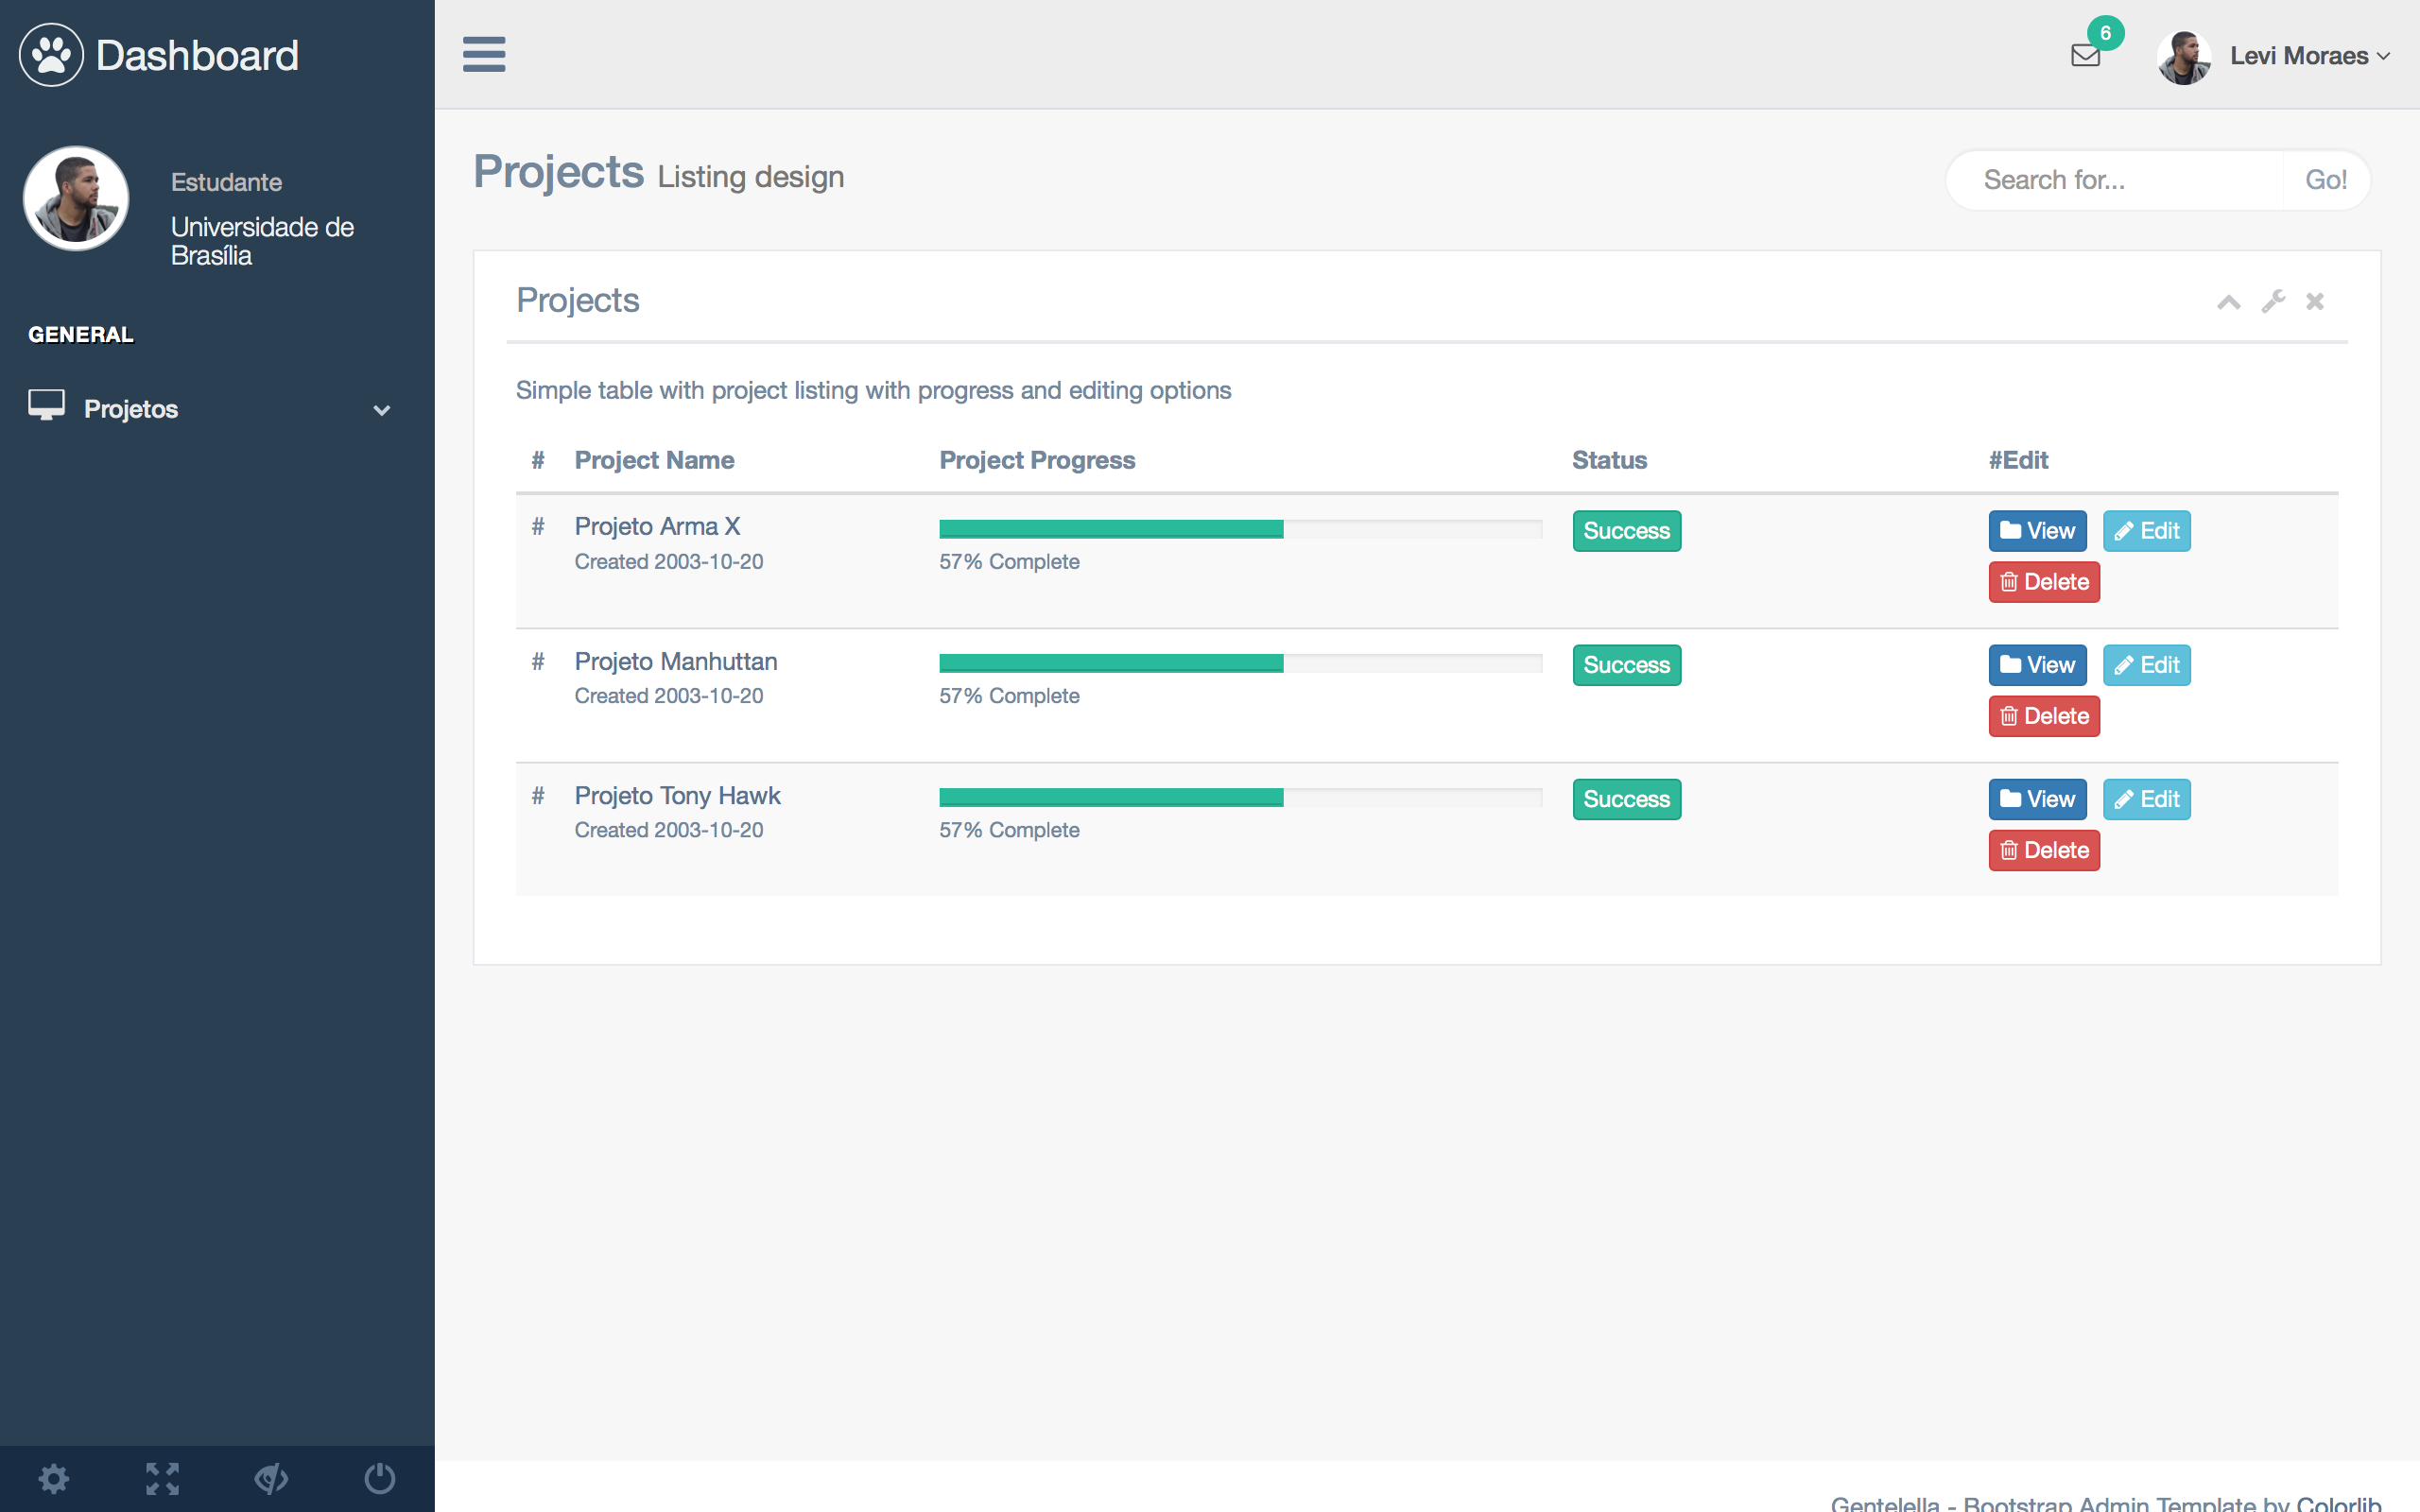
\includegraphics[scale=0.35]{visualizacao_projetos}
\caption{Página de Visualização de Projetos}
\label{img:pag_visual}
\end{figure}

A Figura \ref{img:pag_calendario} apresenta uma funcionalidade que foi sugerida por um dos entrevistados. Está funcionalidade não havia sido planejada inicialmente, mas por ser uma possível necessidade de um cliente, optou-se pela implementação. Ela consiste em um calendário onde e possível acompanhar as datas de inicio e fim de um projeto, assim como possíveis reuniões com a equipe de desenvolvimento.

\graphicspath{{figuras/}}
\begin{figure}[h]
\centering
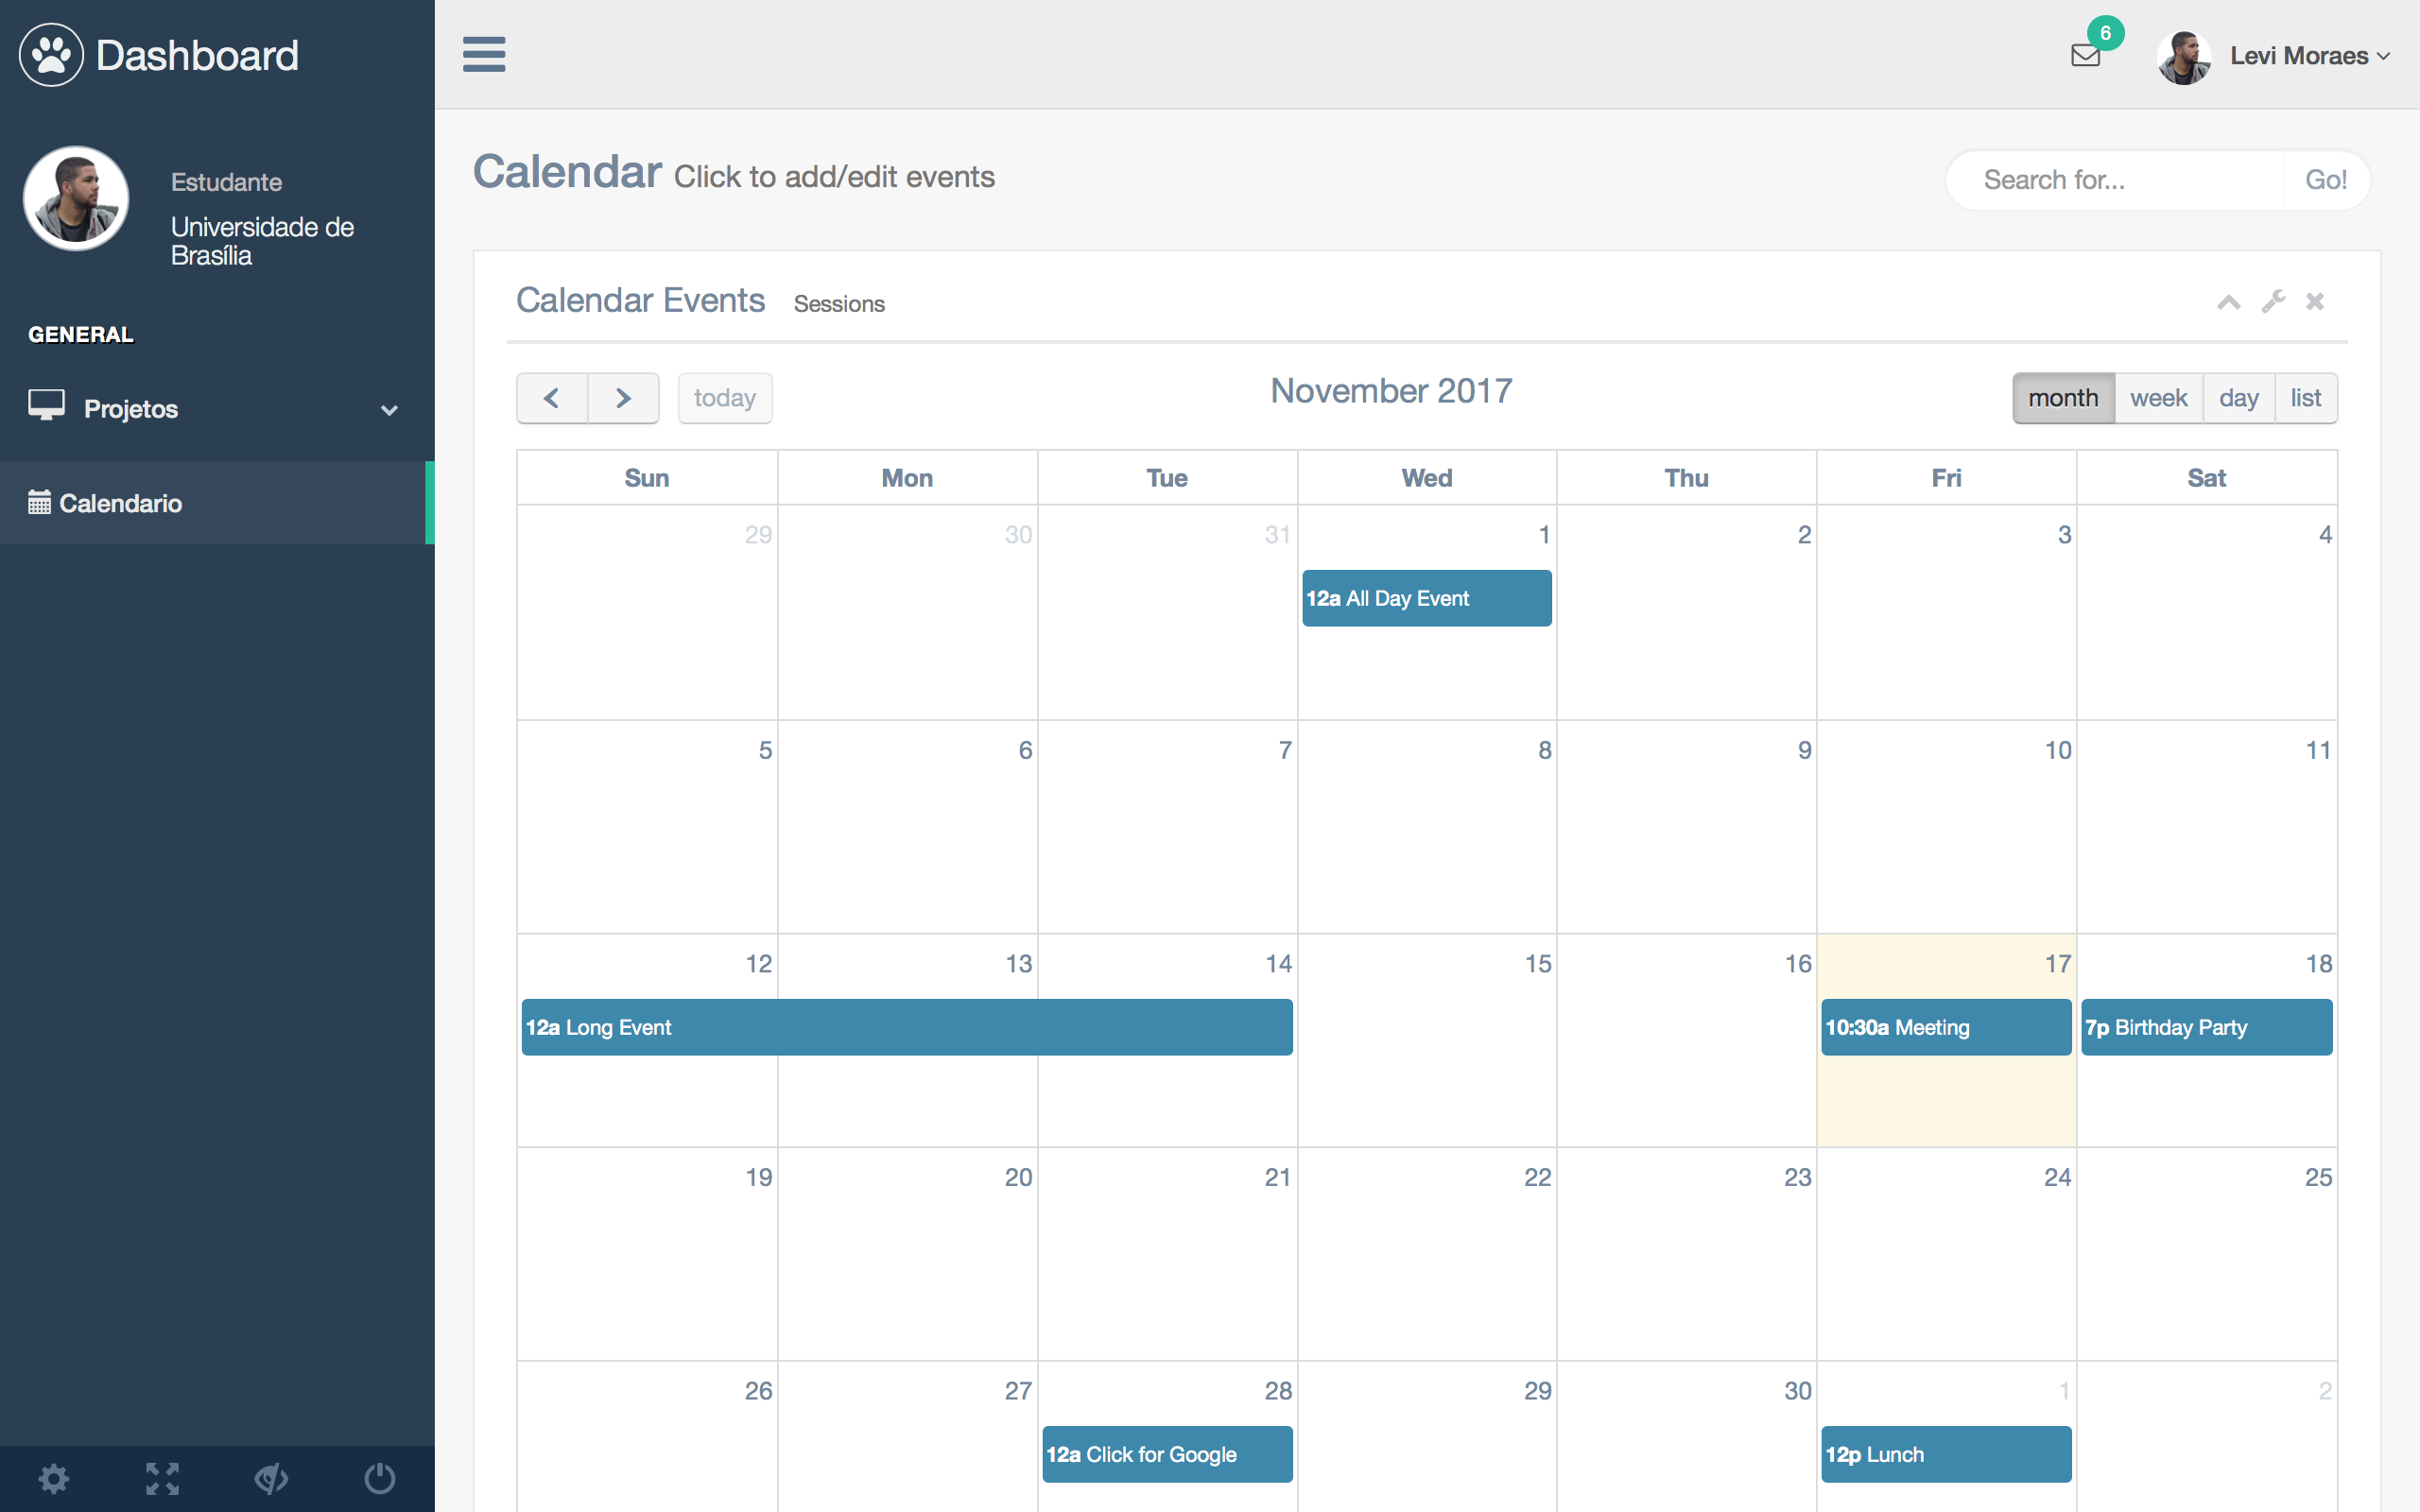
\includegraphics[scale=0.35]{calendario}
\caption{Página de Calendário da Aplicação}
\label{img:pag_calendario}
\end{figure}

A terceira \textit{sprint} tinha como principal objetivo implementar uma tela em que fosse possível adicionar novas ferramentas de análise estática. O software funciona nativamente com o SonarQube, para está funcionalidade implementou-se a analise através da ferramenta Codacy. A Figura \ref{pag_conf} apresenta a página onde é adicionada uma nova ferramenta. Nesta página é necessário dizer o nome da ferramenta e adicionar um arquivo na linguagem Python com as instruções da ferramenta. Para que a ferramenta seja incorporada à analise do \textit{dashboard}, é necessário que no arquivo Python em que é submetido ao software atenda os seguintes critérios:

\begin{itemize}
\item A ferramenta deve ser capaz de inserir no banco de dados todas as métricas que serão utilizadas pela ferramenta.
\item A ferramenta deve prover uma descrição de cada métrica.
\item A ferramenta deve indicar o endereço onde se encontra cada métrica.
\end{itemize} 

\graphicspath{{figuras/}}
\begin{figure}[h]
\centering
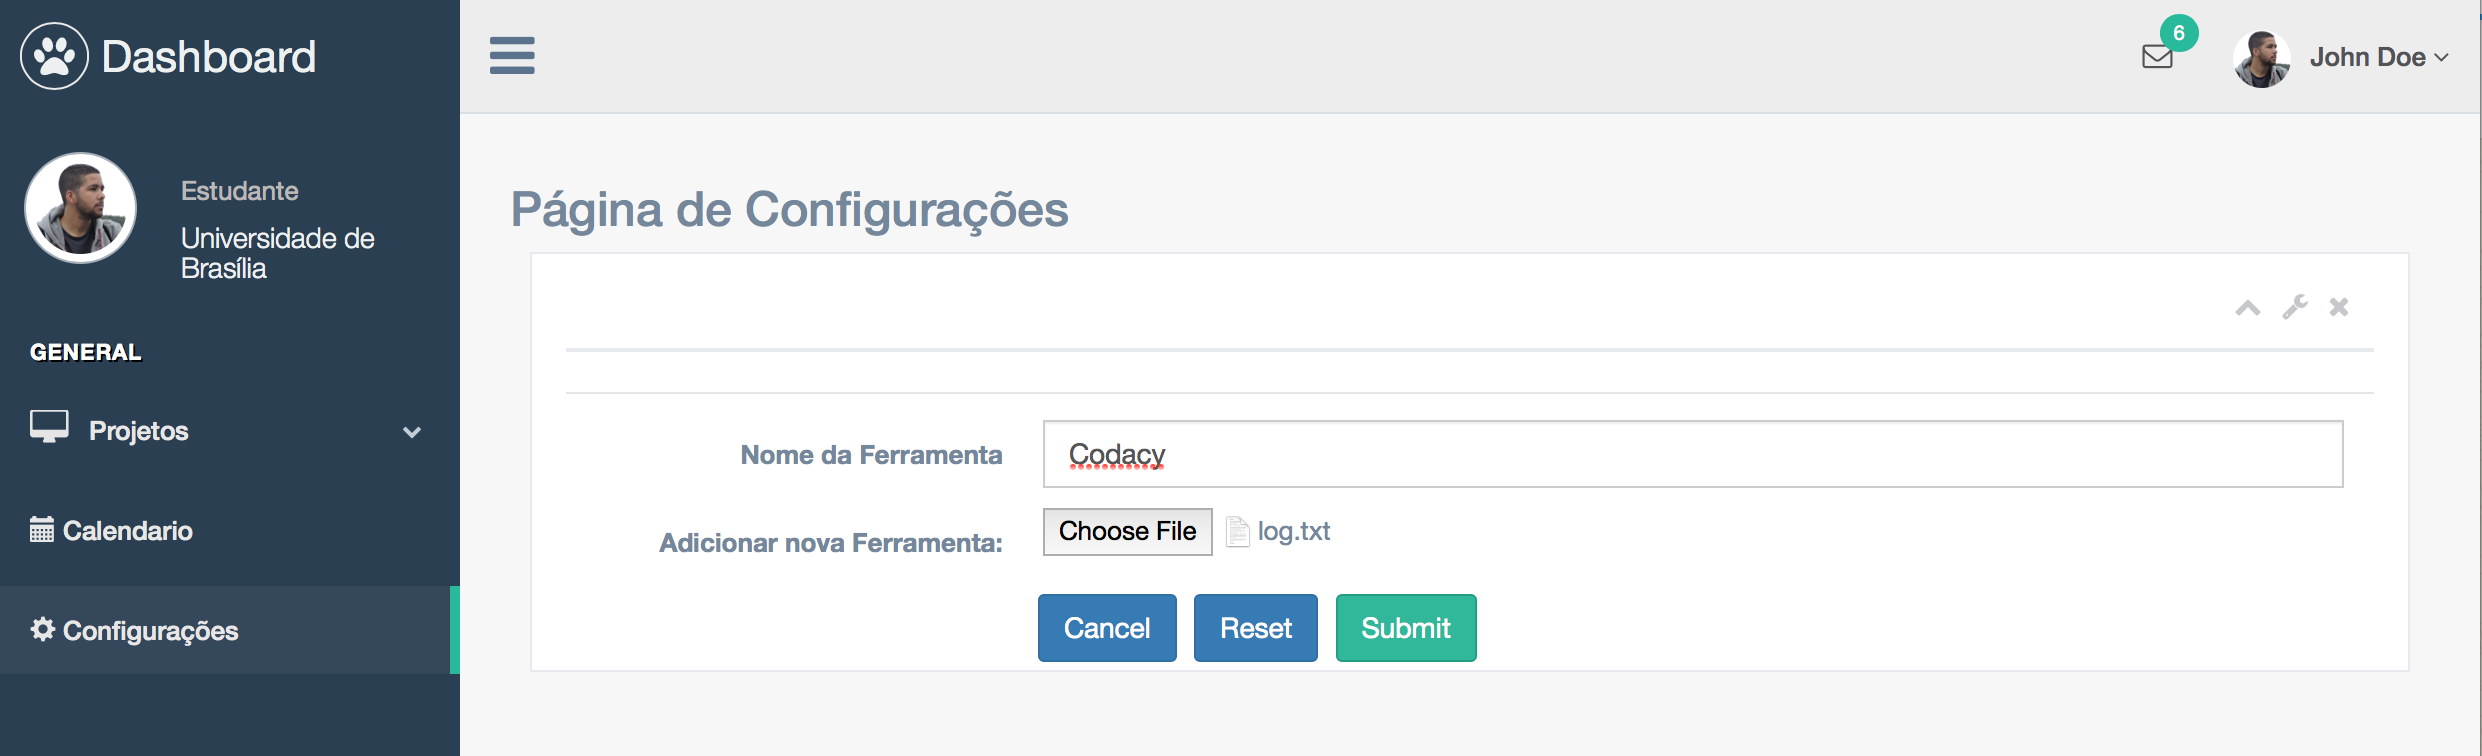
\includegraphics[scale=0.40]{pagina_configuracao.png}
\caption{Página de Configuração da Aplicação}
\label{pag_conf}
\end{figure}


A quarta e última \textit{sprint} consistia na implementação da funcionalidade de Criar Módulo de Sugestão de Métricas. Para implementar essa função optou-se pela implementação de uma solução em Python que compara o perfil do gestor que está cadastrando um projeto com outros quatro perfis de gestores. Devido ao fato de não ter havido interesse por parte de gestores reais, optou-se pelo uso de Personas para simular os quatro gestores. A primeira persona criada é o Excesso. Excesso possui um perfil mais voltado para gestores que preferem o excesso de métricas à insuficiência de informação. A segunda \textit{Persona} é o Novato. O perfil de Novato é semelhante ao de um gestor mais inexperiente, e que não sabe ainda quais métricas são mais importantes para cada tipo de projeto, por isso o valor alto na maioria das métricas escolhidas. O Mínimo possui um perfil voltado para gestores que só desejam as informações essenciais, as métricas desse perfil tendem a ser métricas que impactam diretamente na usabilidade da ferramenta. Por último, o Ingênuo é uma simulação de um gestor que é inexperiente e ao mesmo tempo não conhece muitas das métricas e por isso avalia somente as que conhece. A Figura \ref{img:tabela_notas} ilustra um quadro com as métricas e as notas das métricas atribuídas a cada \textit{Persona}. 


\graphicspath{{figuras/}}
\begin{figure}[h]
\centering
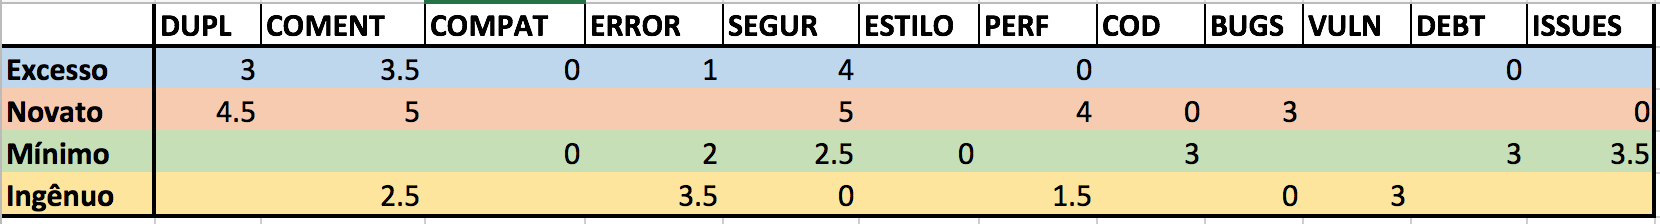
\includegraphics[scale=0.60]{tabela_de_usuarios.png}
\caption{Tabela de Notas por Métrica Atribuído a Cada Persona}
\label{img:tabela_notas}
\end{figure}

Com o término da quarta \textit{sprint} realizou-se a ultima iteração do teste de usabilidade, que consistia na realização de um questionário seguindo o modelo SUS para avaliação do software por parte dos usuários. O resultado do questionário e apresentado na Tabela \ref{tbl:questionario}. Os resultados foram coletados de forma que não fosse possível identificar as notas que cada usuário definiu. Seguindo a forma de pontuação do SUS as perguntas 1,3 e 5 foram subtraídos 1 do valor aferido enquanto que das perguntas foi subtraído 5 do valor coletado. 

\begin{table}[h!]
\centering
\caption{Tabela de Resultados do Questionário SUS}
\label{tbl:questionario}
\begin{tabular}{ll}
\textbf{}               & \textbf{Nota} \\
\textbf{Entrevistado 1} & 80          \\
\textbf{Entrevistado 2} & 82.5            \\
\textbf{Entrevistado 3} & 72.5            \\
\textbf{Entrevistado 4} & 90          \\
\textbf{Entrevistado 5} & 50          \\
\textbf{Entrevistado 6} & 92.5            \\
\textbf{Entrevistado 7} & 70          \\
\rowcolor[HTML]{34CDF9} 
\textbf{Média Geral}    & 76.78        
\end{tabular}
\end{table}

O valor médio de 76.78 representa um valor aceitável dado que a nota máxima que é possível alcançar no teste é 100. Um dos motivos ao qual se acredita a boa nota, se deve ao fato, de que algumas das perguntas do questionário estavam diretamente relacionadas à aplicabilidade do software no uso cotidiano, o que para três dos sete entrevistados faz parte da sua realidade.



\section{Resumo}
Foram realizadas um total de quatro \textit{sprints} para desenvolver todo o \textit{dashboard}. Ao fim das \textit{sprints} um e dois, foram realizados testes de usabilidade com um grupo de sete usuários, neste teste eram coletados dados referentes à experiência na utilização da ferramenta quanto ao domínio da ferramenta. Juntamente com os testes de usabilidade, também era feita uma entrevista de maneira informal com o intuito de outras possíveis melhorias. Na última \textit{sprint} foi realizado o teste de usabilidade SUS com os entrevistados, obteve-se o resultado de 76.78 que é um resultado aceitável, levando em consideração que o teste não foi aplicado unicamente com possíveis usuários.